\chapter{Part 4c. Instruction Level Parallelism}
In the last chapter, we've seen how pipelining can make it easier to parallelize indepent operations making it the overall process faster.

\subsection{Pipelining the Processor}
Pipelining in processors is a technique that splits the execution of an instruction into multiple stages, each handled in parallel by separate hardware units. By doing so, multiple instructions can be processed simultaneously, thereby increasing the overall throughput of the processor without increasing the clock frequency.

\begin{itemize}
    \item[-] \textbf{Fetch (F)}: Retrieve the instruction from memory (often from the instruction cache).
    \item[-] \textbf{Decode (D)}: Interpret the fetched instruction, identify operands, and configure the control signals for execution.
    \item[-] \textbf{Execute (E)}: Perform the required operations (e.g., arithmetic, logic, load, store).
\end{itemize}

\noindent In a basic pipeline with three stages (F, D, E), each stage takes one clock cycle. While one instruction is being executed, a second instruction can be decoded, and a third can be fetched at the same time. This overlapping of tasks leads to a substantial improvement in instruction throughput.

\subsubsection*{Example Pipeline Schedule}
Consider a schedule where three instructions (\(i\), \(i+1\), and \(i+2\)) enter the pipeline. Each instruction occupies a unique pipeline stage in any given clock cycle. Figure~\ref{fig:pipeline-schedule} illustrates how each instruction advances one stage every cycle:
\[
\begin{array}{c|cccccc}
\text{Time} & t & t+1 & t+2 & t+3 & t+4 & t+5 \\ \hline
i     & F & D & E & - & - & - \\
i+1   & - & F & D & E & - & - \\
i+2   & - & - & F & D & E & - \\
\end{array}
\]

\subsubsection*{Multi-Cycle Processor vs.\ Pipelined Processor}
A \emph{multi-cycle} processor might use multiple cycles to execute every instruction (e.g., separate cycles for Fetch, Decode, ALU, Memory Access, and Write Back), but only one instruction flows through the processor at a time. In contrast, a \emph{pipelined} processor allows the next instruction to begin its Fetch stage in parallel with the Decode stage of the previous instruction, greatly improving throughput.
\begin{center}
    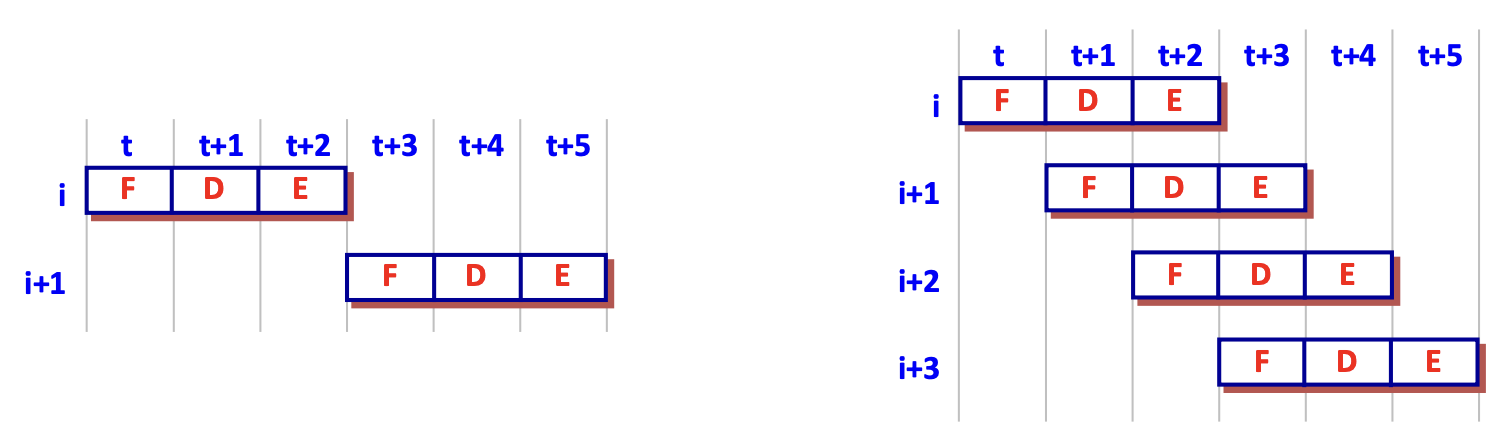
\includegraphics[width=0.65\textwidth]{chapters/chapter4c/images/vs.png}
\end{center}
\subsubsection*{Key Observations for Pipelining}
\begin{enumerate}
    \item \textbf{Repetitive Activity}: Pipelining is effective only when the processor has a large number of instructions to execute.
    \item \textbf{Subactivities}: Each major task (Fetch, Decode, Execute, etc.) should be clearly separable into sub-stages to allow parallel operation.
    \item \textbf{Throughput Gain}: Once the pipeline is full, an instruction completes at the end of every cycle (in the ideal case), increasing throughput.
\end{enumerate}

\noindent Properly designing pipeline stages and handling hazards (such as data, control, and structural hazards) ensures that the pipeline delivers high performance without correctness issues.

\section{Hardware Reuse Across Processor Stages}

In processor design, the approach to hardware reuse varies significantly between multicycle and pipelined architectures. Understanding these differences is crucial for optimizing performance and resource utilization.

\subsection{Multicycle Processor Architecture}

A multicycle processor divides instruction execution into distinct \textbf{states}, allowing certain hardware components to be shared across these states. This sharing is feasible because the components are not required simultaneously, enabling efficient resource utilization.

\begin{itemize}
    \item \textbf{FETCH} State: Typically involves an \textit{adder} to increment the program counter (PC).
    \item \textbf{EXECUTE} State: Requires an \textit{Arithmetic Logic Unit} (ALU) to perform operations.
\end{itemize}

Since the \textit{adder} and the \textit{ALU} are not active concurrently, the ALU can be repurposed to increment the PC during the FETCH state. This reuse reduces the overall hardware complexity and cost.

\subsection{Pipelined Processor Architecture}

In contrast, a pipelined processor operates with multiple \textbf{stages} that are active simultaneously. Each stage performs a different part of the instruction execution process, necessitating dedicated hardware for each stage to avoid conflicts and ensure seamless parallelism.

\begin{itemize}
    \item All pipeline stages are \textit{active concurrently}, handling different instructions in each stage.
    \item Hardware components cannot be shared across stages since multiple instructions require access to the same resources simultaneously.
    \item Consequently, hardware must be \textit{replicated} where necessary to maintain pipeline efficiency and prevent bottlenecks.
\end{itemize}

The inability to share hardware across pipeline stages often leads to increased hardware requirements compared to multicycle processors. However, this replication is essential for achieving high instruction throughput and maximizing pipeline performance.
\newpage
\section{Two Main Challenges in Processor Design}

Designing efficient processors involves addressing several challenges. Two prominent issues are the \textbf{CISC vs. RISC} debate and \textbf{instruction independence}.

\subsection{CISC vs. RISC}
\begin{enumerate}
    \item \textbf{Pipeline Efficiency in CISC vs. RISC}
    \begin{itemize}
        \item[] \textbf{Question}: Can we construct a pipeline for a Complex Instruction Set Computer (CISC) that matches the efficiency of a pipeline designed for a Reduced Instruction Set Computer (RISC)?
        \item[] \textbf{Implications}:
        \begin{itemize}
            \item RISC architectures typically use simpler, fixed-length instructions, which are easier to pipeline efficiently.
            \item CISC architectures have more complex, variable-length instructions, potentially complicating pipeline design and reducing efficiency.
            \item The distinction influences processor complexity, performance, and power consumption.
        \end{itemize}
    \end{itemize}
    \item \textbf{Ensuring Correct Execution with Dependent Instructions}
    \begin{itemize}
        \item \textbf{Issue}: Instructions are often \textit{dependent} on the results of preceding instructions, violating the assumption of \textbf{instruction independence}.
        \item \textbf{Challenge}: Executing code correctly in the presence of such dependencies requires soxphisticated mechanisms to handle hazards, such as data forwarding or pipeline stalls.
    \end{itemize}
\end{enumerate}

Addressing instruction dependencies is critical for maintaining the integrity of program execution while striving for optimal pipeline performance. Techniques such as out-of-order execution and speculative execution are often employed to mitigate the impact of these dependencies.
\section{Multi-Cycle Execution Using an FSM}
In a multi-cycle processor design, each instruction's execution is broken down into multiple steps (states), and the processor transitions through these steps via an FSM.

\subsection{FSM vs.\ Pipeline}
While a pipeline has a fixed sequence of stages (fetch, decode, execute, memory, writeback) for any instruction, an FSM-based multi-cycle design can assign different numbers of steps to each instruction. The FSM transitions vary based on the instruction being executed.



\subsection{Adding Instructions in a Multi-Cycle Design}
When introducing new instructions (e.g., \texttt{lw} or \texttt{add}), the FSM must be extended to accommodate additional states. For example, \texttt{lw} requires computing the address and accessing memory, whereas \texttt{add} mainly requires using the ALU to perform arithmetic. \\
\begin{minipage}[t]{0.45\textwidth}
\textbf{Adding \texttt{add} instruction}\\
We can support the \texttt{add} operation without changing drastically the design, we just need to add it to the ALU.
\[
\text{Fetch} \; \rightarrow \; \text{Decode} \; \rightarrow \; \text{Execute} \; \rightarrow \; \text{Writeback}.
\]
\end{minipage}
\hfill
\vline
\hfill
\begin{minipage}[t]{0.45\textwidth}
\textbf{Adding \texttt{lw} instruction}\\
However, for supporting \texttt{lw} instruction, we need to introduce \textbf{memory} to our design, so we add new steps.
\[
\text{Fetch} \; \rightarrow \; \text{Decode} \; \rightarrow \; \text{Execute} \; \rightarrow \; \text{Memory} \; \rightarrow \; \text{Writeback}.
\]
\end{minipage}
\newpage

\subsection{Adding Instructions to a Pipelined Processor}
Let's look at how this looks like in a pipelined processor.\\
\textit{In this example, we suppose xor and add instructions are both well supported.}
\begin{center}
    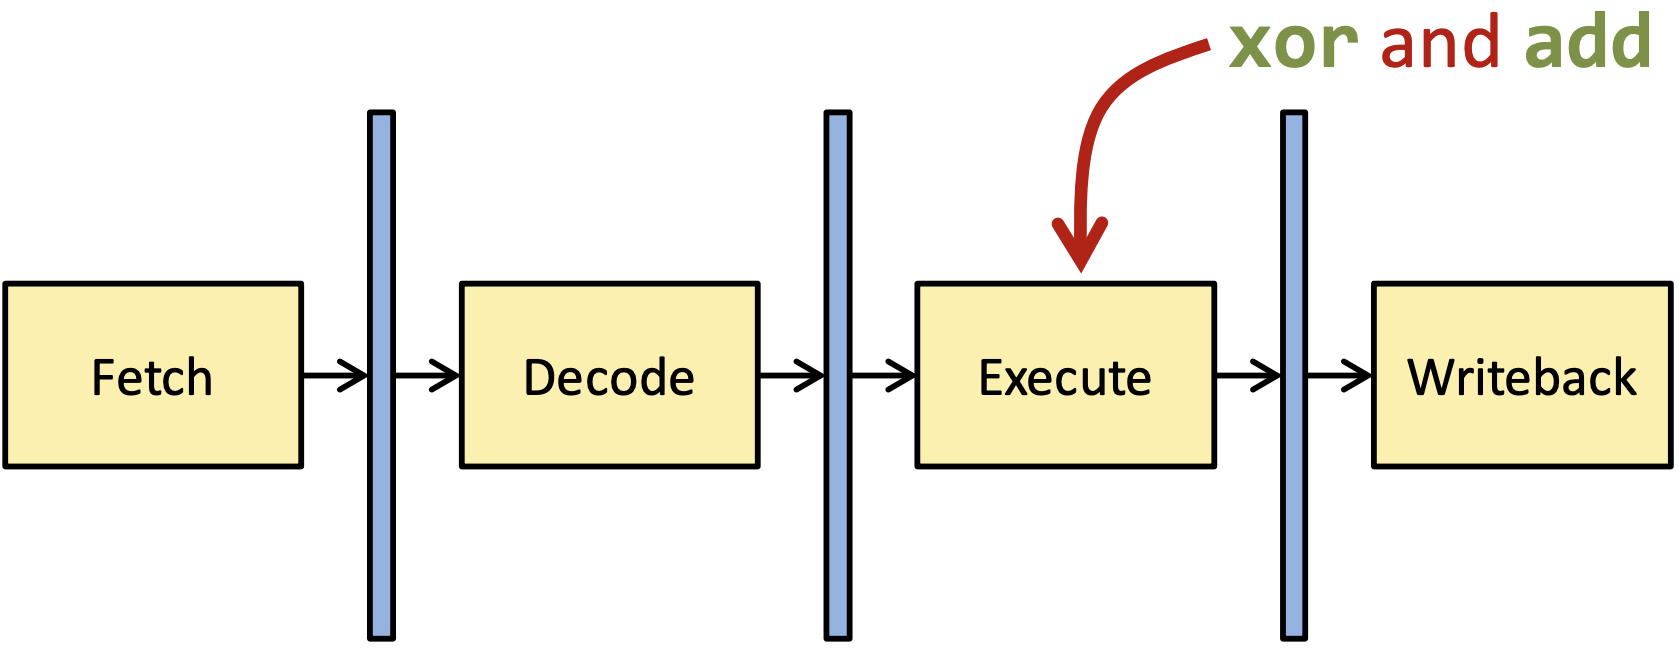
\includegraphics[width=0.45\textwidth]{chapters/chapter4c/images/pipelined-proc.png}
\end{center}
Now, to support \texttt{lw} instruction, we need to add a memory steps, the problem here is that, in a pipelined processor, changes affect \textbf{all instructions}, meaning that now, an \texttt{add} instruction will also take 5 cycles to complete. Thus,
\begin{center}
    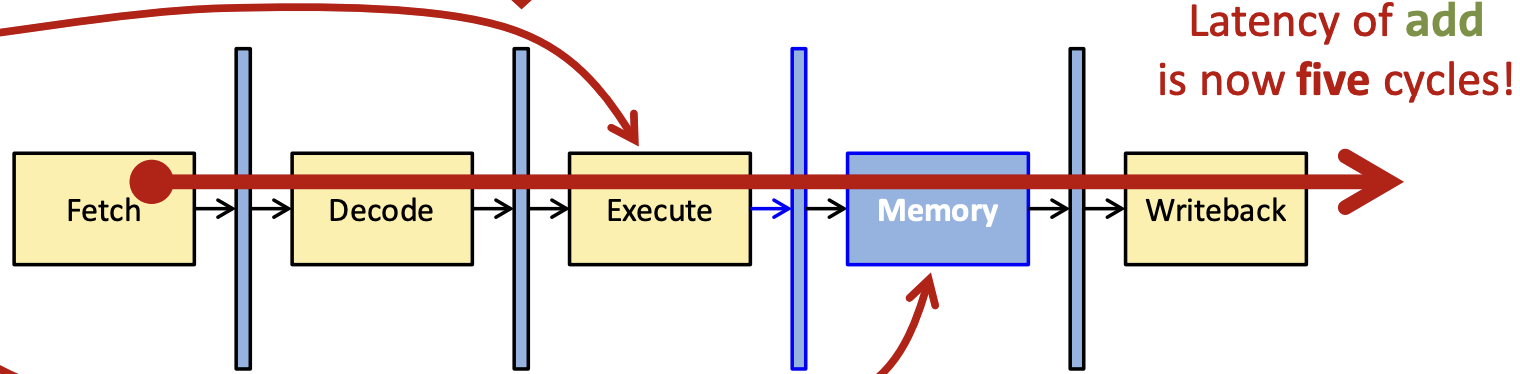
\includegraphics[width=0.45\textwidth]{chapters/chapter4c/images/pipelined-proc-lw.png}
\end{center}

\section{The Importance of the ISA (CISC vs.\ RISC)}
The Instruction Set Architecture (ISA) heavily influences how instructions map onto hardware. A single complex CISC instruction might perform multiple memory accesses and arithmetic operations. In contrast, a RISC instruction set typically emphasizes simplicity: each instruction performs a smaller, more uniform set of operations.

\subsection{A CISC Example}
Consider a hypothetical CISC instruction:
\[
\texttt{sub 8(t4), 0(t1), 0(t2)}
\]
This single instruction might:
\begin{enumerate}
    \item Read the value in memory at address \(\texttt{t2 + 0}\).
    \item Read another value in memory at address \(\texttt{t1 + 0}\).
    \item Subtract these two values.
    \item Finally, store the result in memory at address \(\texttt{t4 + 8}\).
\end{enumerate}
Such complexity can inflate pipeline latency for \emph{all} instructions if the pipeline must accommodate these multi-step operations within a single instruction.
\begin{center}
    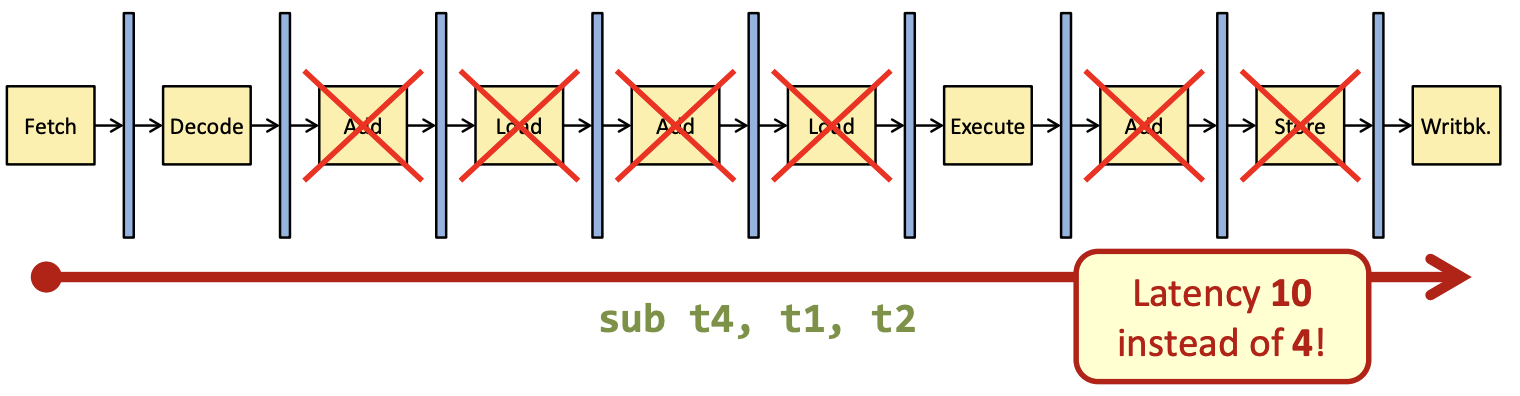
\includegraphics[width=0.65\textwidth]{chapters/chapter4c/images/cisc.png}
\end{center}
\subsection{The RISC Alternative}

Instead of imposing a \textbf{huge penalty} to every simple instruction by making complex instructions possible, the RISC approach advocates for \textbf{only using similarly simple instructions} and building programs with these. \\
\begin{minipage}[htp]{0.45\textwidth}
    \begin{center}
        \begin{tabular}{c c c}
        \texttt{sub 8(t4), 0(t1), 0(t2)} & $\longrightarrow$ &
        \begin{minipage}{0.45\linewidth}
        \texttt{lw t3, 0(t1)} \\
        \texttt{lw t5, 0(t2)} \\
        \texttt{sub t3, t3, t5} \\
        \texttt{sw t3, 8(t4)}
        \end{minipage} \\
        \end{tabular}
        \end{center}
\end{minipage}
\hfill
\vline
\hfill
\begin{minipage}[htp]{0.45\textwidth}
    It turns out that while this is not the only approach, \textbf{it is a good one}, and we will follow it in this course. \\
    In practice, modern CPUs blend design philosophies, using pipelining and other advanced techniques while balancing the complexities of their ISAs. A clear understanding of these concepts---from how an FSM handles instruction steps to how a pipeline benefits from simpler instructions---is crucial to mastering processor design.
\end{minipage}

\subsection{MIPS Pipelining Example}

The MIPS architecture uses a 5-stage pipeline to execute instructions. These stages are: Fetch (F), Decode (D), Execute (E), Memory (M), and Writeback (W). Each instruction moves through these stages, enabling the overlapping of instruction execution, which improves performance by allowing multiple instructions to be processed simultaneously.
\begin{center}
    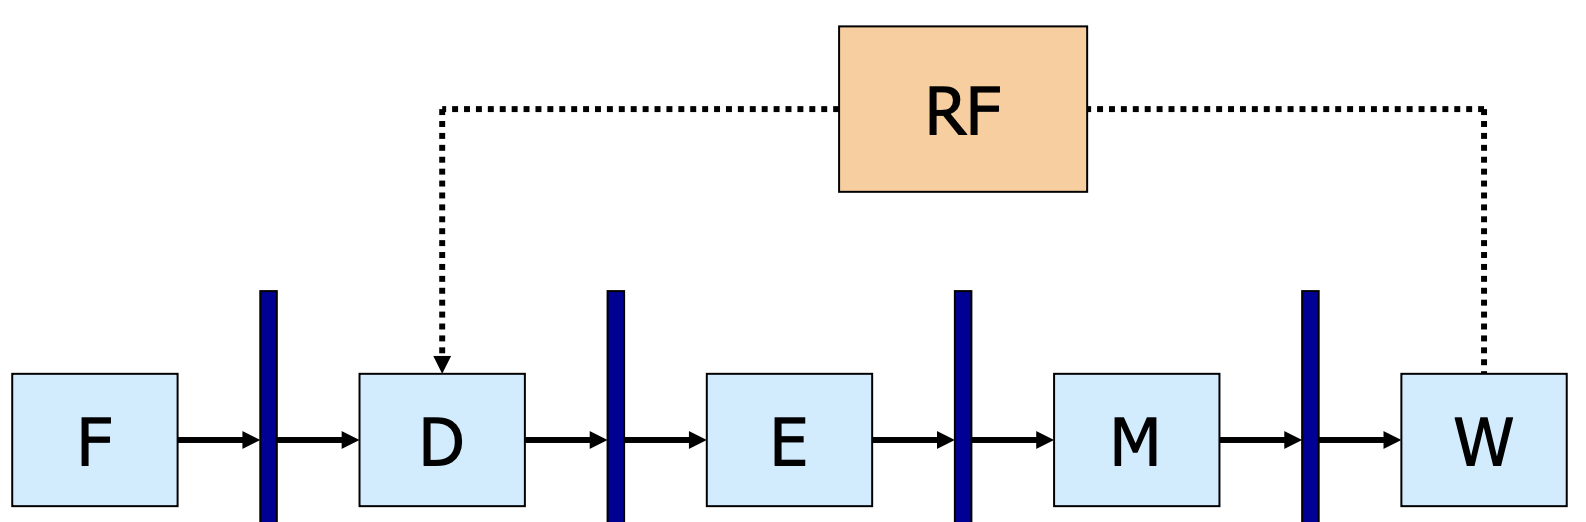
\includegraphics[width=0.45\textwidth]{chapters/chapter4c/images/pipelined-mips.png}
\end{center}
\begin{enumerate}
    \item \textbf{Fetch (F):} The instruction is fetched from the instruction memory.
    \item \textbf{Decode (D):} The instruction is decoded, and the required arguments are obtained from the register file.
    \item \textbf{Execute (E):} The required operation is performed in the Arithmetic Logic Unit (ALU), including address calculations for loads and stores.
    \item \textbf{Memory (M):} Access to data memory is performed if needed, particularly for load and store operations.
    \item \textbf{Writeback (W):} The result of the operation, whether from the ALU or memory, is written back to the register file.
\end{enumerate}

This pipelining model allows instructions to be executed in parallel, thus improving the throughput of the processor and allowing more efficient use of system resources.

\subsection{The Laundry Metaphor for Pipelining}
Pipelining in computer architecture can be explained using the laundry metaphor. Consider the tasks involved in doing laundry: washing, drying, folding, and putting away. Each of these steps represents a stage in the pipeline.
\begin{center}
    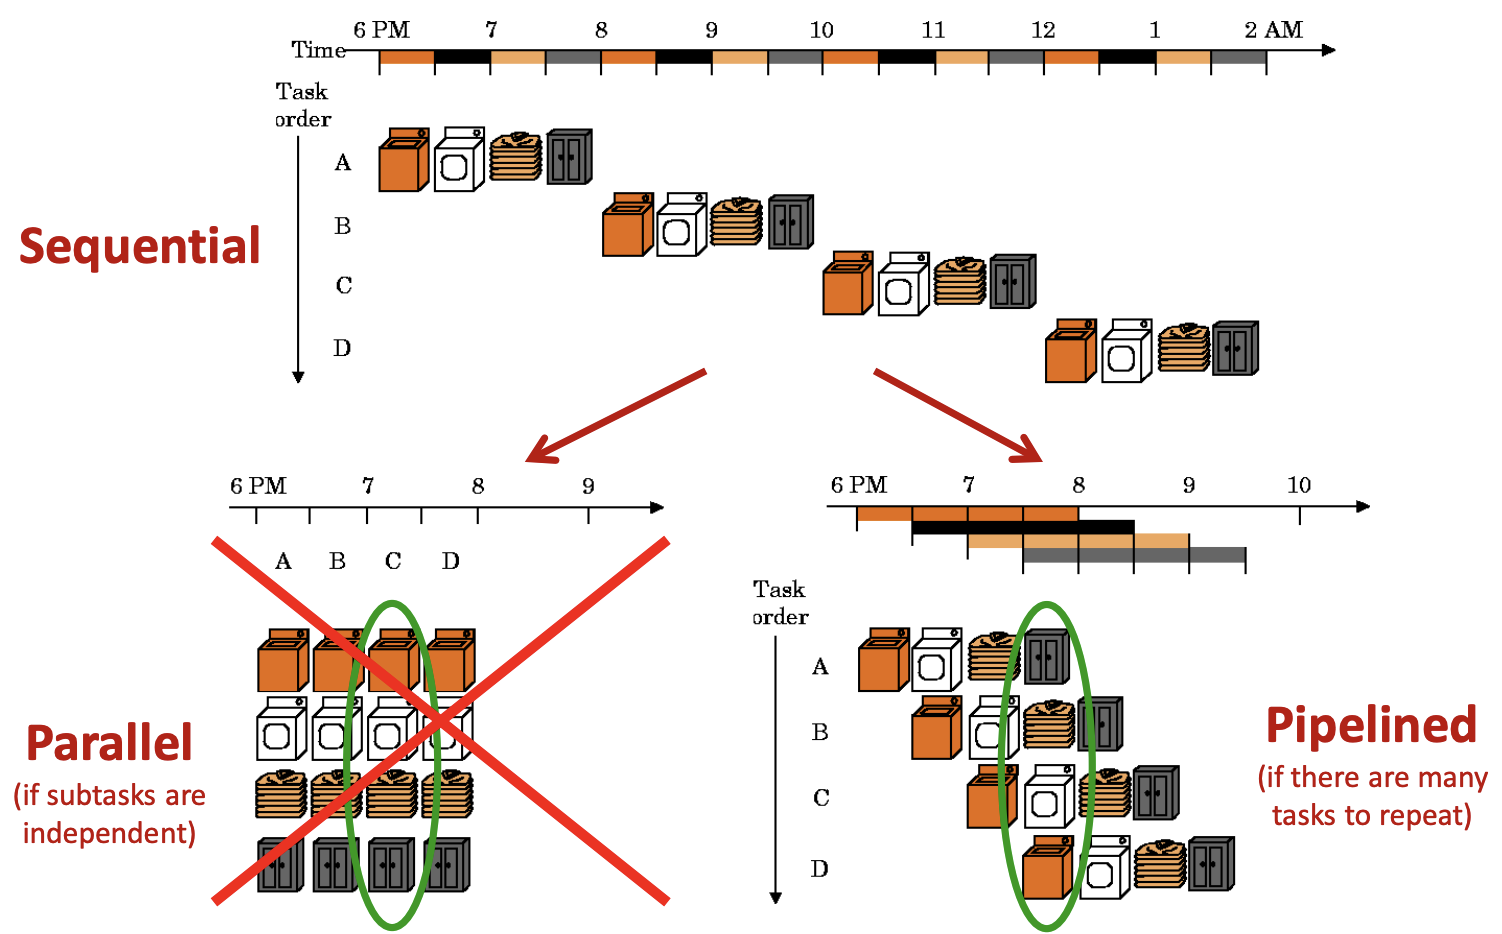
\includegraphics[width=0.65\textwidth]{chapters/chapter4c/images/laundry.png}
\end{center}
\begin{itemize}
    \item[-] \textbf{Sequential Execution:} In a sequential process, one load of laundry is completed through all stages before starting the next. This approach takes a long time because each load must wait for the previous one to finish.
    \item[-] \textbf{Parallel Execution:} If the subtasks are completely independent, multiple washing machines, dryers, and folders could be used simultaneously. However, this is often impractical due to resource limitations.
    \item[-] \textbf{Pipelined Execution:} In pipelining, multiple loads of laundry are processed simultaneously, with each load at a different stage. For example, while one load is being washed, another is dried, and a third is folded. This overlaps the tasks, significantly reducing total time.
\end{itemize}

\newpage
\subsection{Two Distinct Memory Interfaces in MIPS}

In a MIPS processor, two distinct memory interfaces are utilized to enhance performance by allowing concurrent operations: the 	extbf{Instruction Cache} and the 	extbf{Data Cache}. These interfaces are depicted in the following architecture:
\begin{center}
    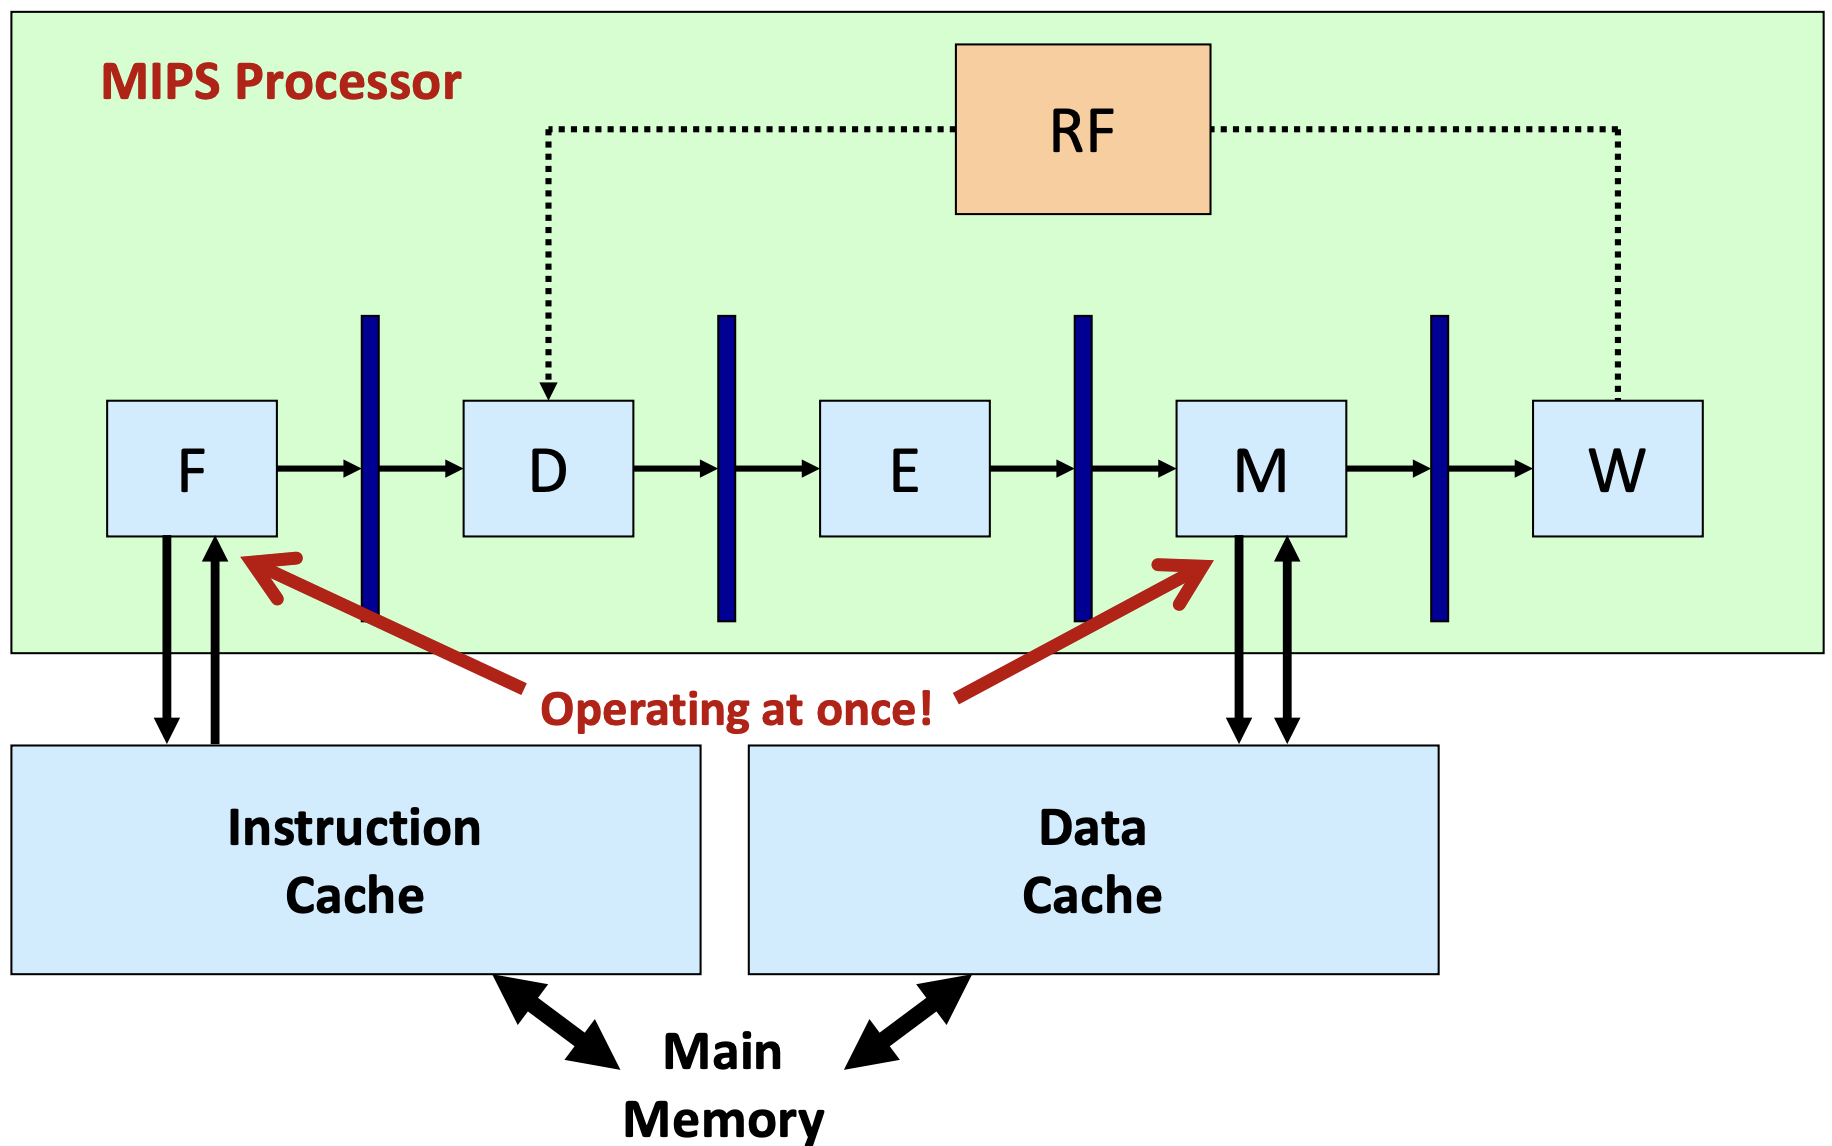
\includegraphics[width=0.45\textwidth]{chapters/chapter4c/images/mips.png}
\end{center}
\begin{itemize}
    \item[-] The \textbf{Instruction Cache} is accessed during the \textbf{Fetch} (F) stage, retrieving instructions for execution.
    \item[-] The \textbf{Data Cache} is utilized during the \textbf{Memory} (M) stage, providing data required for processing.
\end{itemize}

The pipeline stages of the MIPS processor are as follows:
\begin{enumerate}
    \item \textbf{F (Fetch)}: Instructions are fetched from the Instruction Cache.
    \item \textbf{D (Decode)}: Instructions are decoded, and operands are prepared using the Register File (RF).
    \item \textbf{E (Execute)}: The instruction is executed.
    \item \textbf{M (Memory)}: Data is accessed from or written to the Data Cache.
    \item \textbf{W (Write-back)}: Results are written back to the register file.
\end{enumerate}

The separation of memory interfaces allows the Instruction and Data caches to operate simultaneously, enabling improved throughput and reduced bottlenecks in the pipeline. Additionally, the Register File (RF) facilitates data flow between the stages.

This dual-interface approach is critical for high-performance pipelined architectures, allowing overlapping of instruction fetch and memory access operations.

\subsection{Example of Pipelined Execution }
\href{https://github.com/elazdi-al/comparch/raw/refs/heads/main/chapters/chapter4c/images/video.mp4}{You can view an animation of the execution here.}
